% Robot Description for RoboCup@Home Open Platform League (OPL)
% Team: UruBots (Uruguay)
% Robot: Base@Home

\section*{Robot Hardware Description: Base@Home [OPL]}%
\label{sec:annex-OPL}

\setlength\intextsep{0pt}
\begin{wrapfigure}[12]{r}{0.35\textwidth}
	\centering
	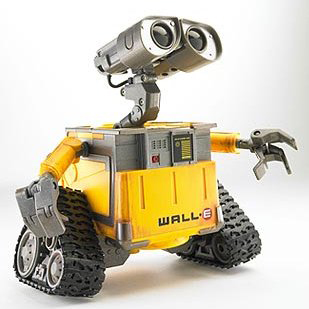
\includegraphics[width=0.33\textwidth]{images/robot.jpg}
	\caption{Base@Home Robot}%
	\label{fig:base_athome}
\end{wrapfigure}

Base@Home is a custom open-platform service robot developed by team UruBots for the RoboCup@Home Open Platform League (OPL). Physical specifications are as follows:

\begin{itemize}
	\item \textbf{Dimensions \& Weight:} Footprint $0.48\,\text{m} \times 0.48\,\text{m}$, chassis height $0.22\,\text{m}$, total height $1.35\,\text{m}$ (RuleBook \S 4.4: width $\le 70\,\text{cm}$, height $\le 200\,\text{cm}$). [TBD \#6: Measured total weight in kg].
	\item \textbf{Base Traction:} Differential-drive chassis ($0.48\,\text{m} \times 0.48\,\text{m}$, clearance $0.04\,\text{m}$). Two repurposed 6.5-inch brushless DC (BLDC) hub motors with Hall-effect sensors (15 pole pairs, 90 ticks/rev, $5.95\,\text{mm}$/tick), effective wheel radius $0.0853\,\text{m}$, track width $0.5620\,\text{m}$, rear passive caster wheel ($r = 0.04\,\text{m}$). STM32F103 motor controller with custom Field-Oriented Control (FOC) firmware~\cite{feru2024hoverboard} over UART at 50\,Hz. Maximum nominal velocity $0.38\,\text{m/s}$.
	\item \textbf{Torso (Pan-Elevation):} $1.30\,\text{m}$ central vertical aluminum profile ($0.06\,\text{m}$ width). NEMA 23 stepper motor (1600 steps/rev, 1/8 microstepping) driven by ESP32-S3 microcontroller with dual debounced hardware limit switches (working stroke $0.60\,\text{m}$, carriage height $0.40$--$1.00\,\text{m}$ above floor). Structural torso prism ($0.25\,\text{m} \times 0.35\,\text{m} \times 0.35\,\text{m}$) carrying a front-facing $0.26\,\text{m} \times 0.18\,\text{m}$ interactive facial display and speaker.
	\item \textbf{Manipulators (1):} Side-mounted AgileX Piper 6-DOF robotic arm ($1.5\,\text{kg}$ payload, $626\,\text{mm}$ reach, parallel two-finger gripper $0$--$95\,\text{mm}$) mounted on left vertical torso face ($+Y$ outward, $-Z$ downward). Shoulder origin at $z = 0.465$--$1.065\,\text{m}$ in base frame. Controlled via SocketCAN at 50\,Hz.
	\item \textbf{Head (Pan-Tilt):} 2-DOF pan-tilt unit driven by Robotis Dynamixel XL430-W250 servos over 1\,Mbaud U2D2 interface (IDs 1 and 2, Protocol 2.0, 20\,Hz).
	\item \textbf{RGB-D Sensors (2):}
		\begin{enumerate*}[label=(\roman*)]
			\item Intel RealSense D435 ($640\times 480$ @ 15\,Hz, firmware 5.17.0.10) mounted on the pan-tilt head;
			\item Orbbec DaBai DC1 ($640\times 480$ @ 15\,Hz) mounted eye-in-hand on the Piper wrist ($25\,\text{mm}$ along $+X$, $56\,\text{mm}$ above approach axis, $80\,\text{mm}$ behind fingertips).
		\end{enumerate*}
	\item \textbf{LiDAR Sensors (1):} Front Hokuyo UST-05LX 2D LiDAR ($270^\circ$ FOV, $0.06$--$5.0\,\text{m}$, 40\,Hz) at $x = 0.22\,\text{m}$, beam height $0.38\,\text{m}$.
	\item \textbf{Microphones (1):} Directional supercardioid shotgun microphone: R\O{}DE VideoMic GO II (USB, 48\,kHz capture downsampled to 16\,kHz) mounted on the head assembly.
	\item \textbf{Other Sensors:} Integrated Hall effect wheel sensors (90 ticks/rev); dual hardware limit switches on torso carriage; CAN feedback on Piper joints and gripper width.
	\item \textbf{Other Actuators:} ESP32-S3 stepper driver; parallel two-finger gripper ($0$--$95\,\text{mm}$).
	\item \textbf{Onboard Computing:}
		\begin{itemize}[nosep]
			\item Primary Host: CHUWI LarkBox S mini-PC (Intel Core i3-1220P 10C/12T, 15\,GiB RAM, 468\,GB NVMe SSD, Ubuntu 24.04.3 LTS, ROS 2 Jazzy). Runs navigation, planning, compiler, local LLM/VLM, and user interfaces.
			\item Secondary Host: NVIDIA Jetson Orin Nano 8\,GB Super Dev Kit (6-core Arm Cortex-A78AE, Ampere GPU, CUDA 13.2, TensorRT 10.16.2, 7.4\,GiB shared RAM, Ubuntu 24.04.4 LTS / JetPack 7.2.1). Runs arm controller, head controller, wrist vision, TensorRT YOLO inference, and streaming Whisper ASR.
		\end{itemize}
	\item \textbf{Internal Network:} Point-to-point 1\,Gbps wired Ethernet link ($0.2\,\text{ms}$ RTT, $\ge 660\,\text{Mbps}$) with unicast CycloneDDS (strictly no WiFi hotspot).
	\item \textbf{Power \& Safety:} [TBD \#7: Battery capacity, nominal voltage, BMS, fuse ratings, and emergency stop button per RuleBook \S 3.3.2].
\end{itemize}

\section*{Robot's Software Description}
\textit{Software packages developed specifically by team UruBots are marked with an asterisk ($^*$):}

\begin{itemize}
	\item \textbf{Audio filtering:} Silero VAD (voice activity detection), directional weak-voice gating ($0.34\,\text{ms}$/block).
	\item \textbf{Automated speech recognition:} \texttt{whisper\_node}$^*$ using \texttt{faster-whisper} (\texttt{base.en} int8 on CPU), request-indexed streaming pipeline, bilingual support.
	\item \textbf{Natural Language Processing:} \texttt{command\_parser.py}$^*$ (deterministic bilingual grammar DAG compiler), \texttt{gpsr\_parser}$^*$ / \texttt{gpsr\_plan.py}$^*$ (official GPSR grammar compiler), \texttt{llm\_intent.py}$^*$ (Qwen2.5 1.5B Q4 grammar-bounded fallback), \texttt{vlm.py}$^*$ / \texttt{vlm\_server.py}$^*$ (SmolVLM 500M Q8 for scene VQA).
	\item \textbf{Navigation, localization, and mapping:} Nav2~\cite{macenski2020marathon2} (AMCL, SmacPlanner2D, RegulatedPurePursuitController, RotationShimController), \texttt{hoverboard\_driver}$^*$, \texttt{front\_dock.py}$^*$ (LiDAR-based frontal docking), \texttt{map\_zone\_editor.py}$^*$ (semantic annotations).
	\item \textbf{Object recognition:} \texttt{bag\_finder.py}$^*$, YOLOv8s-worldv2~\cite{cheng2024yoloworld} open-vocabulary detector with background distractors, wrist DaBai DC1 monocular mid-height raycaster.
	\item \textbf{People recognition:} Face tracking with pan-tilt head; person Re-ID [TBD / future work].
	\item \textbf{People tracking:} YOLOv8n-pose with rolling torso-center tracking, \texttt{follow\_logic.py}$^*$ (distance-bounded person follower).
	\item \textbf{Pose/Gesture recognition:} 3D pointing-gesture localization (\texttt{bag\_vision.py}$^*$ raycasting arm-torso angle $\ge 25^\circ$), customer raised-hand detection (\texttt{raised\_hand.py}$^*$).
	\item \textbf{Manipulation:} \texttt{piper\_arm\_controller.py}$^*$ (50\,Hz SocketCAN with safety guards), \texttt{arm\_manipulation.py}$^*$, MoveIt 2 (TRAC-IK, OMPL multi-orientation planning), \texttt{door\_open.py}$^*$ (lever door opener), \texttt{quest\_teleop\_node.py}$^*$ (WebXR 6D pose Cartesian control).
	\item \textbf{Sound source localization:} None (directional shotgun mic with mechanical pan-tilt orientation).
	\item \textbf{Simulation Stack:} \texttt{base\_athome\_sim}$^*$ (\texttt{sim\_scene.py}$^*$ z-buffer RGB-D visual simulation, \texttt{sim\_arm.py}$^*$, \texttt{sim\_torso.py}$^*$, \texttt{sim\_mic.py}$^*$).
\end{itemize}

\section*{External Devices and Cloud Services}
\begin{itemize}
	\item \textbf{Wireless / Hotspots:} None (strictly zero-hotspot compliance per RuleBook \S 3.2.8~\cite{robocup_rulebook_2026}).
	\item \textbf{External Compute:} None. All planning, vision, ASR, foundation models, and control run 100\% onboard.
	\item \textbf{Development Teleoperation:} Meta Quest 2 headset via wired USB tunnel (\texttt{localhost:8765}).
	\item \textbf{Cloud Services:} None (no off-board or cloud APIs in the operational loop).
\end{itemize}
